\documentclass[12pt,a4paper]{article}
\usepackage[utf8]{inputenc}
\usepackage[vietnamese]{babel}
\usepackage{graphicx}
\usepackage{float}
\usepackage{geometry}
\geometry{a4paper, margin=2.5cm}
\usepackage{hyperref}
\usepackage{xcolor}
\usepackage{fancyhdr}
\usepackage{titlesec}
\usepackage{booktabs}
\usepackage{array}
\usepackage{listings}

\hypersetup{
    colorlinks=true,
    linkcolor=blue,
    filecolor=magenta,      
    urlcolor=cyan,
    pdftitle={Bao cao Bai tap 6 - AI co trach nhiem va dao duc trong hoc tap},
    pdfpagemode=FullScreen,
}

% Cấu hình listings cho code Java
\definecolor{codegreen}{rgb}{0,0.6,0}
\definecolor{codegray}{rgb}{0.5,0.5,0.5}
\definecolor{codepurple}{rgb}{0.58,0,0.82}
\definecolor{backcolour}{rgb}{0.95,0.95,0.92}

\lstdefinestyle{mystyle}{
    backgroundcolor=\color{backcolour},   
    commentstyle=\color{codegreen},
    keywordstyle=\color{magenta},
    numberstyle=\tiny\color{codegray},
    stringstyle=\color{codepurple},
    basicstyle=\ttfamily\footnotesize,
    breakatwhitespace=false,         
    breaklines=true,                 
    captionpos=b,                    
    keepspaces=true,                 
    numbers=left,                    
    numbersep=5pt,                  
    showspaces=false,                
    showstringspaces=false,
    showtabs=false,                  
    tabsize=2
}
\lstset{style=mystyle}

% Cấu hình header & footer
\pagestyle{fancy}
\fancyhf{}
\rhead{Hành trình Kỹ năng số}
\lhead{Bài tập Thực hành 6}
\rfoot{Trang \thepage}

% Định dạng tiêu đề mục
\titleformat{\section}{\normalfont\Large\bfseries\color{blue!80!black}}{\thesection}{1em}{}
\titleformat{\subsection}{\normalfont\large\bfseries\color{blue!60!black}}{\thesubsection}{1em}{}

\begin{document}

% --- TRANG BÌA ---
\begin{titlepage}
    \centering
    \vspace*{1cm}
    
    {\large \bfseries TRƯỜNG ĐẠI HỌC CÔNG NGHỆ - ĐHQGHN} \\[0.2cm]
    {\large \bfseries KHOA CÔNG NGHỆ THÔNG TIN} \\[1.5cm]
    
    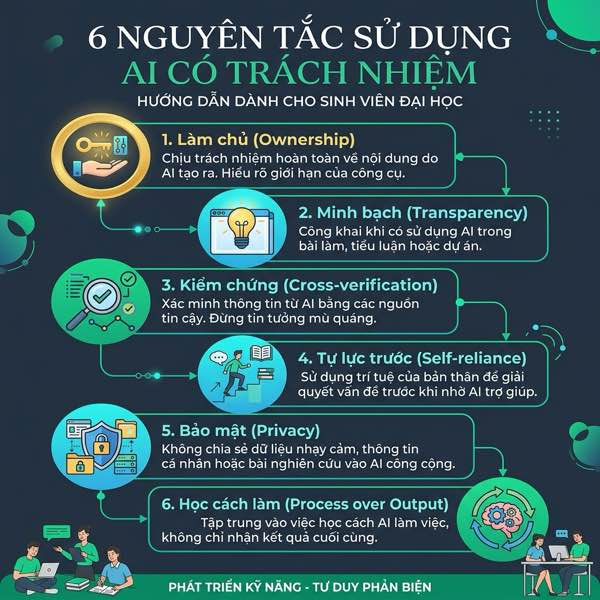
\includegraphics[width=0.45\textwidth]{images/responsible_ai_infographic.jpg} \\[1.0cm]
    
    {\Large \bfseries BÁO CÁO BÀI TẬP THỰC HÀNH CÁ NHÂN} \\[0.5cm]
    {\Large \bfseries BÀI TẬP 6: AI CÓ TRÁCH NHIỆM VÀ ĐẠO ĐỨC} \\
    {\Large \bfseries TRONG HỌC TẬP VÀ NGHIÊN CỨU} \\[1.5cm]
    
    \textbf{Môn học:} Nhập môn Công nghệ số và Ứng dụng Trí tuệ nhân tạo \\
    \textbf{Chủ đề:} Thiết lập bộ nguyên tắc cá nhân và thực tế hỗ trợ học tập của AI \\[2.0cm]
    
    \begin{flushleft}
        \large
        \textbf{Sinh viên thực hiện:} Nguyễn Bảo Đăng \\
        \textbf{Mã số sinh viên:} 25020115 \\
    \end{flushleft}
    
    \vfill
    {\large Năm 2026}
\end{titlepage}

\newpage
\tableofcontents
\newpage

% --- NỘI DUNG CHÍNH ---

\section{Nghiên cứu chính sách của trường đại học về việc sử dụng AI}

Hiện nay, Đại học Quốc gia Hà Nội (VNU) nói chung và Trường Đại học Công nghệ (UET) nói riêng đang có những bước tiến mạnh mẽ trong việc đưa Trí tuệ nhân tạo (AI) vào môi trường học thuật. Bắt đầu từ năm học 2025-2026, VNU đã đưa học phần ``Nhập môn công nghệ số và ứng dụng trí tuệ nhân tạo'' (VNU1001) vào chương trình bắt buộc cho toàn bộ sinh viên năm nhất.

Phân tích các điểm chính trong chính sách và định hướng của VNU:
\begin{enumerate}
    \item \textbf{Chấp nhận và tận dụng (Embrace \& Utilize):} Thay vì cấm đoán, nhà trường hướng tới việc đào tạo sinh viên biết tận dụng AI một cách thông minh, hiệu quả. AI được xem như một công cụ hỗ trợ tư duy sáng tạo, không phải là công cụ để làm hộ.
    \item \textbf{Đề cao tính trách nhiệm và đạo đức:} Các định hướng của VNU đặc biệt nhấn mạnh vào ``công dân số tự tin, trách nhiệm''. Việc sử dụng các mô hình ngôn ngữ lớn (LLMs) trong làm bài tập, viết code, hay nghiên cứu phải đi kèm với khả năng kiểm chứng thông tin và minh bạch trong trích dẫn.
    \item \textbf{Tích hợp đa ngành:} Việc ứng dụng AI không chỉ giới hạn trong nhóm ngành Công nghệ Thông tin mà được lan tỏa ra các môn học khác, đòi hỏi sinh viên phải hiểu rõ lằn ranh giữa việc dùng AI để tham khảo cấu trúc so với việc gian lận học thuật.
\end{enumerate}

\textbf{Nhận định cá nhân:} Chính sách của VNU là một bước đi cực kỳ thức thời và tiến bộ. So với một số trường đại học trên thế giới từng có giai đoạn cấm hoàn toàn ChatGPT, việc VNU chủ động dạy cách dùng AI cho thấy tầm nhìn xa. Tuy nhiên, ranh giới giữa ``hỗ trợ'' và ``phụ thuộc'' đôi khi rất mong manh, đòi hỏi bản thân mỗi sinh viên phải tự xây dựng cho mình một bộ nguyên tắc làm việc nghiêm ngặt.

\newpage
\section{Thực hiện nhiệm vụ học tập với sự hỗ trợ của AI}

\subsection{Lựa chọn nhiệm vụ}
Chuẩn bị tài liệu hướng dẫn nhóm học tập về cách triển khai ``Singleton Pattern'' trong ngôn ngữ lập trình Java, phục vụ cho việc xây dựng kiến trúc hệ thống của một dự án đấu giá trực tuyến.

\subsection{Ghi lại quá trình sử dụng AI}
\textbf{Prompt đã sử dụng trên ChatGPT:}
\\ \texttt{``Đóng vai là một lập trình viên Java Senior. Hãy giải thích ngắn gọn khái niệm Singleton Pattern cho sinh viên năm nhất. Cung cấp 2 đoạn code minh họa trong Java: một đoạn Eager Initialization và một đoạn Thread-safe Lazy Initialization (dùng Double-Checked Locking). Giải thích rủi ro của từng phương pháp.''}

\begin{figure}[H]
    \centering
    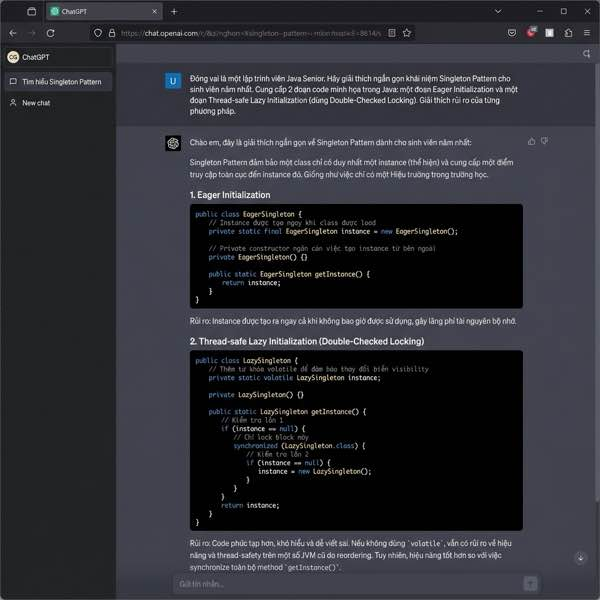
\includegraphics[width=0.75\textwidth]{images/chatgpt_singleton.jpg}
    \caption{Tương tác với ChatGPT để lấy mã nguồn mẫu cho Singleton Pattern}
    \label{fig:chatgpt_prompt}
\end{figure}

\textbf{Đầu ra của AI (Tóm tắt):} AI đã trả về đúng hai đoạn mã nguồn Java theo yêu cầu, kèm theo giải thích rằng Eager Initialization có thể gây lãng phí bộ nhớ nếu object không bao giờ được dùng đến, trong khi Double-Checked Locking thì an toàn trong môi trường đa luồng (multi-thread) nhưng phức tạp hơn.

\subsection{Đánh giá, chỉnh sửa và tích hợp}
\begin{itemize}
    \item \textbf{Đánh giá:} Mã nguồn AI cung cấp chuẩn cú pháp và chạy được. Tuy nhiên, phần giải thích hơi khô khan và mang tính lý thuyết hàn lâm, chưa thực sự phù hợp với văn văn phong chia sẻ nội bộ của nhóm sinh viên.
    \item \textbf{Chỉnh sửa:} Tôi đã kiểm thử (test) lại đoạn code Thread-safe bằng cách chạy thử nhiều luồng trong IntelliJ IDEA để xác thực tính đồng bộ (Hình \ref{fig:intellij_test}). Sau đó, tôi viết lại phần giải thích khái niệm bằng lời văn của mình, lấy ví dụ thực tế liên quan đến việc quản lý kết nối Database trong hệ thống đấu giá để nhóm dễ hiểu hơn.
\end{itemize}

\begin{figure}[H]
    \centering
    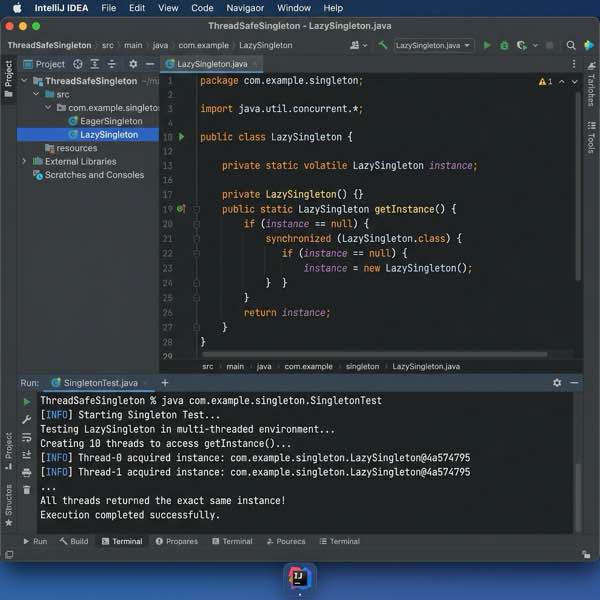
\includegraphics[width=0.75\textwidth]{images/intellij_singleton.jpg}
    \caption{Kiểm thử đoạn mã nguồn Thread-safe trong môi trường IntelliJ IDEA}
    \label{fig:intellij_test}
\end{figure}

\begin{itemize}
    \item \textbf{Tích hợp:} Mã nguồn được đưa vào tài liệu hướng dẫn trên Notion của nhóm. Những phần lý thuyết cơ bản được giữ lại theo dàn ý của AI.
\end{itemize}

\subsection{Trích dẫn minh bạch}
Trong tài liệu của nhóm trên Google Docs, tôi đã chèn một chú thích rõ ràng ở đầu trang để đảm bảo tính trung thực (Hình \ref{fig:docs_citation}):
\\ \textit{``Tài liệu này được biên soạn với sự hỗ trợ của mô hình ngôn ngữ Gemini nhằm tạo khung cấu trúc và mã nguồn cơ sở. Toàn bộ mã nguồn đã được người viết kiểm thử thực tế và tinh chỉnh để phù hợp với kiến trúc dự án.''}

\begin{figure}[H]
    \centering
    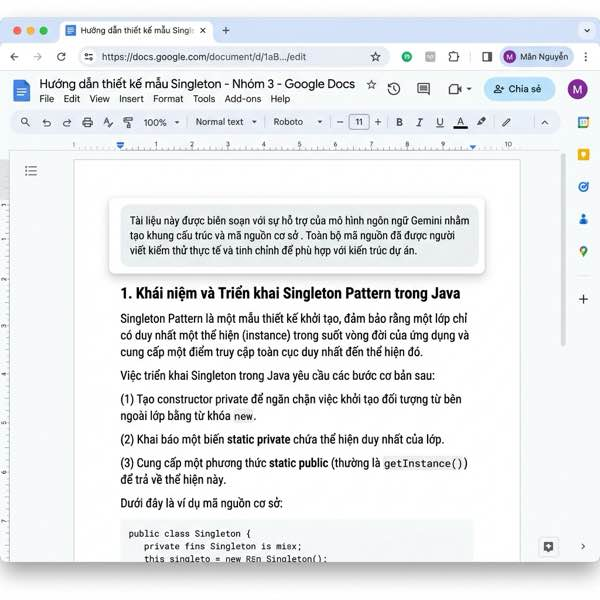
\includegraphics[width=0.8\textwidth]{images/docs_citation.jpg}
    \caption{Chú thích trích dẫn việc sử dụng AI minh bạch trên Google Docs}
    \label{fig:docs_citation}
\end{figure}

\newpage
\section{Phân tích các vấn đề đạo đức khi sử dụng AI trong học thuật}

\begin{itemize}
    \item \textbf{Ranh giới giữa hỗ trợ hợp lý và gian lận học thuật:} Đây là vấn đề nhức nhối nhất. Việc sử dụng AI để gợi ý cấu trúc một bài luận, tìm ra lỗi sai trong một đoạn code, hoặc tóm tắt tài liệu vật lý phức tạp là ``hỗ trợ hợp lý''. Nó giống như việc bạn hỏi bài một gia sư. Tuy nhiên, việc sao chép toàn bộ đoạn văn hay mã nguồn do AI tạo ra và nộp dưới tên mình (pass off as one's own) chính là gian lận. Ranh giới này nằm ở ``tính nguyên bản của giá trị cốt lõi'' -- tư duy và quyết định cuối cùng phải thuộc về con người.
    
    \item \textbf{Vấn đề về quyền sở hữu trí tuệ và trích dẫn:} Các AI hiện tại được huấn luyện dựa trên khối lượng dữ liệu khổng lồ từ internet, bao gồm cả các tác phẩm có bản quyền. Khi AI tạo ra một đoạn code tối ưu hay một giáo án hay, câu hỏi đặt ra là: Ai sở hữu nó? Việc trích dẫn AI không giống như trích dẫn một tác giả cụ thể, mà là việc minh bạch quy trình làm việc. Nếu sinh viên không trích dẫn việc dùng AI, họ đang vi phạm đạo đức học thuật về sự trung thực.
    
    \item \textbf{Tác động đến quá trình học tập và phát triển kỹ năng:}
    \begin{itemize}
        \item \textit{Tác động tích cực:} AI cá nhân hóa quá trình học. Khi giải các bài tập tự nhiên hóc búa, sinh viên có thể yêu cầu AI giải thích từng bước thay vì chỉ xin đáp án, từ đó tăng tốc độ hiểu bài.
        \item \textit{Tác động tiêu cực:} Việc lạm dụng AI tạo ra ``sức ỳ nhận thức'' (cognitive offloading). Nếu gặp một bug code hoặc một phương trình khó mà lập tức nhờ AI giải quyết, sinh viên sẽ mất đi kỹ năng tư duy phản biện (critical thinking) và khả năng chịu đựng áp lực khi giải quyết vấn đề (problem-solving resilience). Về lâu dài, điều này làm thui chột năng lực thực chất.
    \end{itemize}
\end{itemize}

\newpage
\section{Xây dựng bộ nguyên tắc cá nhân (6 nguyên tắc sử dụng AI)}

Để sử dụng AI một cách có trách nhiệm, bản thân tôi luôn tuân thủ nghiêm ngặt hệ thống 6 nguyên tắc cốt lõi sau:

\begin{figure}[H]
    \centering
    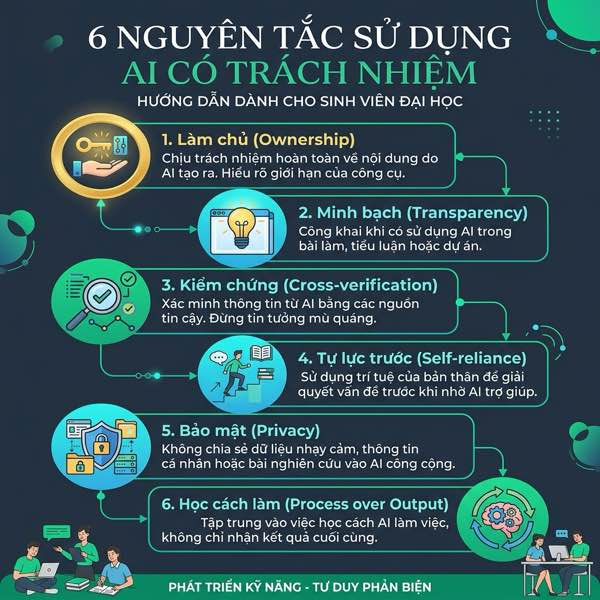
\includegraphics[width=0.65\textwidth]{images/responsible_ai_infographic.jpg}
    \caption{Infographic 6 nguyên tắc sử dụng AI có trách nhiệm}
    \label{fig:responsible_ai_poster}
\end{figure}

\begin{enumerate}
    \item \textbf{Nguyên tắc làm chủ (Ownership):} Tư duy và quyết định cuối cùng phải là của tôi. AI đóng vai trò là ``người đồng cấp'' (pair-programmer) hoặc trợ lý, không phải là người quyết định thay.
    \item \textbf{Nguyên tắc minh bạch tuyệt đối (Transparency):} Luôn có dòng ghi chú rõ ràng về việc sử dụng công cụ AI nào, vào mục đích gì (tạo ý tưởng, sửa lỗi ngữ pháp, hay viết code cơ sở) trong mọi sản phẩm học thuật hay dự án nhóm.
    \item \textbf{Nguyên tắc kiểm chứng chéo (Cross-verification):} Không tin tưởng 100\% vào AI (đặc biệt là để tránh hiện tượng AI Hallucination). Mọi số liệu, lý thuyết khoa học, hay logic thuật toán AI cung cấp đều phải được kiểm tra lại qua giáo trình chính thống hoặc tài liệu đối chứng tin cậy.
    \item \textbf{Nguyên tắc ``Tự lực trước, AI sau'':} Khi gặp một vấn đề khó, bắt buộc phải dành ít nhất 15-30 phút tự tư duy và tìm giải pháp. Chỉ khi thực sự bế tắc mới sử dụng AI để xin gợi ý (hint), tuyệt đối không xin đáp án hoàn chỉnh ngay từ đầu.
    \item \textbf{Nguyên tắc bảo mật thông tin (Data Privacy):} Tuyệt đối không đưa các thông tin cá nhân nhạy cảm, mã nguồn độc quyền của các dự án đang phát triển (như private repository), hoặc dữ liệu mật của tổ chức vào các prompt của AI công cộng.
    \item \textbf{Nguyên tắc học cách làm, không học kết quả (Process over Output):} Khi sử dụng AI để sửa một đoạn văn hay tối ưu code, tôi sẽ dành thời gian phân tích tại sao AI lại sửa như vậy, để nâng cao kỹ năng thực tế của bản thân chứ không chỉ đơn thuần sao chép kết quả.
\end{enumerate}

\newpage
\section{Kết luận}

Trí tuệ nhân tạo là một trợ lý vô song mở ra nhiều cơ hội nâng cao hiệu suất trong học tập và nghiên cứu. Tuy nhiên, AI chỉ nên đóng vai trò là điểm bắt đầu hoặc chất xúc tác. Bản sắc thực sự và uy tín học thuật của mỗi cá nhân nằm ở việc làm chủ tri thức, sử dụng công nghệ một cách trung thực, minh bạch và có trách nhiệm đạo đức cao.

\end{document}
